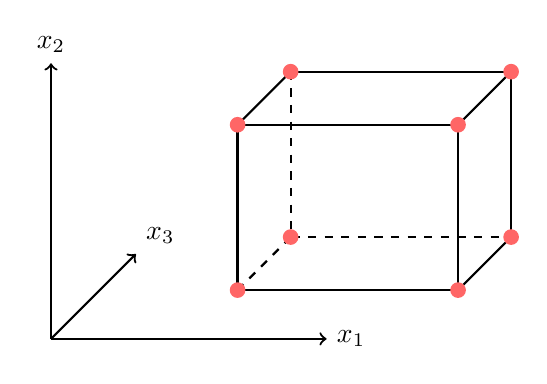
\begin{tikzpicture}[scale = 0.7,
    vertex/.style={circle, fill=red!60, inner sep=2pt},
    edge/.style={thick}
]

% Coordinates of the cuboid
\coordinate (O)   at (3,0.5,-1);
\coordinate (A)   at (7,0.5,-1);
\coordinate (B)   at (7,3.5,-1);
\coordinate (C)   at (3,3.5,-1);

\coordinate (O1)  at (3,0.5,-3.5);
\coordinate (A1)  at (7,0.5,-3.5);
\coordinate (B1)  at (7,3.5,-3.5);
\coordinate (C1)  at (3,3.5,-3.5);

% Coordinate axes
\draw[->, thick] (0,0,0) -- (5,0,0) node[right] {$x_1$};
\draw[->, thick] (0,0,0) -- (0,5,0) node[above]  {$x_2$};
\draw[->, thick] (0,0,0) -- (0,0,-4) node[above right] {$x_3$};

% Cuboid edges
\draw[edge] (O)  -- (A)  -- (B)  -- (C)  -- cycle;
\draw[edge, dashed] (C1) -- (O1) -- (A1);
\draw[edge] (A1) -- (B1) -- (C1);

\draw[edge, dashed] (O)  -- (O1);
\draw[edge] (A)  -- (A1);
\draw[edge] (B)  -- (B1);
\draw[edge] (C)  -- (C1);

% Mark all 8 vertices
\foreach \p in {O,A,B,C,O1,A1,B1,C1}
    \node[vertex] at (\p) {};

% Vertex labels
% \node[below left]  at (O)  {$v_1$};
% \node[below]       at (A)  {$v_2$};
% \node[right]       at (B)  {$v_3$};
% \node[left]        at (C)  {$v_4$};

% \node[left]        at (O1) {$v_5$};
% \node[below right] at (A1) {$v_6$};
% \node[right]       at (B1) {$v_7$};
% \node[left]        at (C1) {$v_8$};

% \node[left]        at (-2,2.5,0) {$P(x_1,x_2,x_3) = \ldots + 5x_1x_2x_3 + \dots$};

\end{tikzpicture}